\documentclass{scrartcl}
\usepackage[utf8]{inputenc}
\usepackage{tikz}
\begin{document}
\subsubsection*{Entscheidungsbaum Totalausfall Netz an einem Rechner}
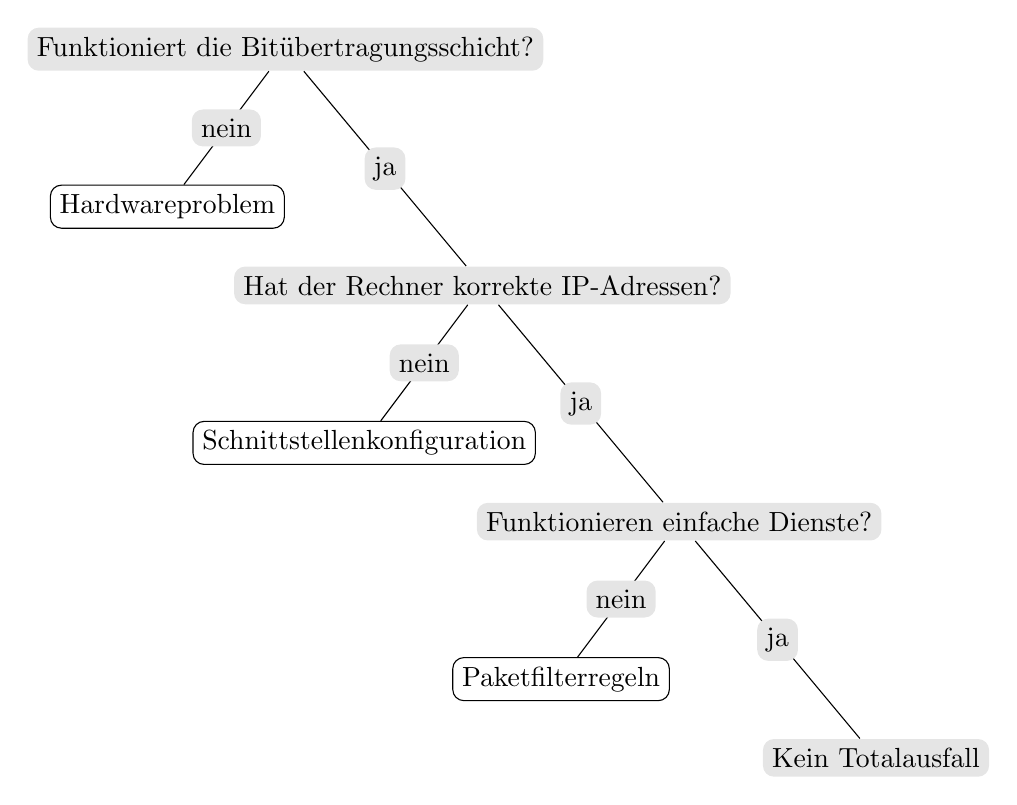
\begin{tikzpicture}
[every node/.style={fill=black!10,rounded corners,align=center},
grow=south, level distance=2cm,
level 1/.style={sibling distance=3cm},
level 2/.style={sibling distance=3cm},
]

\node{Funktioniert die Bitübertragungsschicht?}
  child{node[draw,fill=white]{Hardwareproblem}
  edge from parent node[fill=black!10]{nein}}
  child{node at +(1,-1) {Hat der Rechner korrekte IP-Adressen?}
    child{node[draw,fill=white]{Schnittstellenkonfiguration}
    edge from parent node{nein}}
    child{node at +(1,-1) {Funktionieren einfache Dienste?}
      child{node[draw,fill=white]{Paketfilterregeln}
      edge from parent node{nein}}
      child{node at +(1,-1) {Kein Totalausfall}
      edge from parent node{ja}}
    edge from parent node{ja}}
  edge from parent node{ja}};
\end{tikzpicture}
\end{document}
